% !TeX root = ../main.tex
\chapter{Unidad 2: Leyes de la mecánica clásica y de la termodinámica}
\label{chap:unidad-2}

\section{Propósito y resultados de aprendizaje}
\label{sec:u2-proposito}

Esta unidad estudia cómo las fuerzas modifican el movimiento y cómo la energía se almacena, se transfiere y se disipa. Estos principios permiten construir modelos sencillos de sistemas acústicos y auditivos sin confundir una magnitud física con una sensación sonora. El desarrollo prepara el estudio de las oscilaciones de la Unidad~\ref{chap:unidad-3}; la anatomía y la transducción auditiva se retomarán en las unidades posteriores.

Al finalizar la unidad se espera que sea posible:

\begin{itemize}
    \item interpretar las tres leyes de Newton e identificar el sistema sobre el que actúan las fuerzas;
    \item relacionar fuerza neta, masa, aceleración e inercia mediante un modelo unidimensional;
    \item explicar el papel de la masa, la elasticidad y el amortiguamiento en un sistema mecánico;
    \item distinguir energía cinética, energía potencial elástica, transferencia y disipación;
    \item diferenciar temperatura, calor, energía interna y entropía;
    \item explicar, bajo hipótesis declaradas, por qué la temperatura modifica la velocidad de propagación del sonido en un gas;
    \item aplicar estos conceptos a ejemplos introductorios vinculados con la membrana timpánica, la cadena osicular, un vibrador óseo, los tejidos y la propagación en aire.
\end{itemize}

\section{Conocimientos previos}
\label{sec:u2-previos}

Se utilizarán masa, aceleración, fuerza, presión y velocidad de propagación según las definiciones de la Unidad~\ref{chap:unidad-1}. También se aplicarán conversión de unidades, notación científica y análisis dimensional. No se requiere cálculo diferencial: cuando una magnitud varíe con el tiempo, se interpretará primero su significado físico y luego se presentará la notación necesaria.

\section{Una membrana sometida a una diferencia de presión}
\label{sec:u2-situacion}

Consideremos una membrana flexible que separa dos regiones de aire. Si la presión es igual a ambos lados, las fuerzas debidas a la presión pueden equilibrarse. Si aparece una diferencia de presión, la membrana experimenta una fuerza neta y comienza a acelerarse. Su movimiento posterior no depende solamente de esa fuerza: también intervienen su inercia, su elasticidad y los mecanismos que disipan energía.

Este modelo no reproduce todos los detalles de la membrana timpánica. Su utilidad consiste en organizar preguntas físicas: ¿qué sistema se analiza?, ¿qué fuerzas actúan?, ¿qué propiedad se opone al cambio de movimiento?, ¿qué fuerza tiende a recuperar la posición de equilibrio? y ¿por qué la vibración disminuye cuando cesa la excitación?

\section{Las leyes de Newton}
\label{sec:u2-newton}

\subsection{Sistema, interacción y fuerza neta}
\label{sec:u2-sistema-fuerza}

Antes de aplicar una ley de Newton es necesario elegir el \textbf{sistema}: el cuerpo o conjunto de cuerpos cuyo movimiento se desea describir. Una fuerza representa una interacción entre el sistema y su entorno o entre partes del sistema. La fuerza es una magnitud vectorial; por lo tanto, posee módulo, dirección y sentido.

En un problema unidimensional se elige un sentido positivo y se suman las componentes de las fuerzas con sus signos. La \textbf{fuerza neta}, que se denotará \(F_\mathrm{neta}\) y se medirá en newtons (\(\text{N}\)), es el resultado de esa suma.

\subsection{Primera ley: inercia}
\label{sec:u2-primera-ley}

En un sistema de referencia inercial, un cuerpo mantiene su estado de reposo o de movimiento rectilíneo uniforme cuando la fuerza neta sobre él es nula. Si \(v\) representa la velocidad del cuerpo, medida en metros por segundo (\(\text{m}/\text{s}\)), entonces \(F_\mathrm{neta}=0\) implica que \(v\) permanece constante.

La \textbf{inercia} es la propiedad por la cual un cuerpo se opone a cambios de su velocidad. La masa cuantifica esta propiedad: a igualdad de fuerza neta, un cuerpo de mayor masa cambia su velocidad más lentamente.

La primera ley no explica por qué una membrana desplazada vuelve a su posición de equilibrio. Ese retorno requiere una fuerza neta restauradora, debida a la elasticidad. Además, para que la oscilación disminuya con el tiempo debe existir amortiguamiento.

\subsection{Segunda ley: fuerza neta y aceleración}
\label{sec:u2-segunda-ley}

Sea \(m\) la masa del sistema, medida en kilogramos (\(\text{kg}\)), y sea \(a\) su aceleración en la dirección analizada, medida en metros por segundo cuadrado (\(\text{m}/\text{s}^{2}\)). Para un sistema de masa constante, la segunda ley de Newton se escribe:

\begin{equation}
    F_\mathrm{neta}=ma.
    \label{eq:u2-segunda-ley}
\end{equation}

La ecuación~\eqref{eq:u2-segunda-ley} no afirma que una fuerza produzca velocidad de manera directa: una fuerza neta produce aceleración, es decir, un cambio de velocidad. Si varias fuerzas se equilibran, el sistema puede estar en reposo o moverse con velocidad constante.

\subsubsection*{De la presión a la fuerza sobre una superficie}

La presión y la fuerza no son la misma magnitud. Consideremos una superficie plana de área \(A\), medida en metros cuadrados (\(\text{m}^{2}\)), con presiones uniformes \(p_1\) y \(p_2\) a cada lado, medidas en pascales (\(\text{Pa}\)). Si ambas presiones actúan perpendicularmente a la superficie, la diferencia de presión es:

\[
    \Delta p=p_1-p_2,
\]

donde \(\Delta p\) se mide en pascales. La componente de la fuerza neta debida a esa diferencia es:

\begin{equation}
    F_\mathrm{pres}=\Delta p\,A.
    \label{eq:u2-presion-fuerza}
\end{equation}

El análisis dimensional confirma que:

\[
    \text{Pa}\cdot\text{m}^{2}
    =\frac{\text{N}}{\text{m}^{2}}\cdot\text{m}^{2}
    =\text{N}.
\]

La figura~\ref{fig:u2-fuerza-area} representa las fuerzas opuestas debidas a
presiones uniformes. La flecha neta no representa la presión: representa la
fuerza resultante después de considerar la diferencia de presión y el área.

\begin{figure}[htbp]
    \centering
    % Propósito: distinguir presión de fuerza y mostrar cómo una diferencia de
% presión uniforme sobre un área produce una fuerza neta.
% Origen: Delta p=p_1-p_2 y F_pres=Delta p A, ecuación
% \eqref{eq:u2-presion-fuerza}. Esquema cualitativo, no a escala.
% Descripción accesible: una superficie vertical de área A separa dos regiones.
% La presión p_1 del lado izquierdo empuja hacia la derecha y la presión p_2
% del lado derecho empuja hacia la izquierda. Cuando p_1 es mayor que p_2, la
% fuerza neta F_pres apunta hacia la derecha.
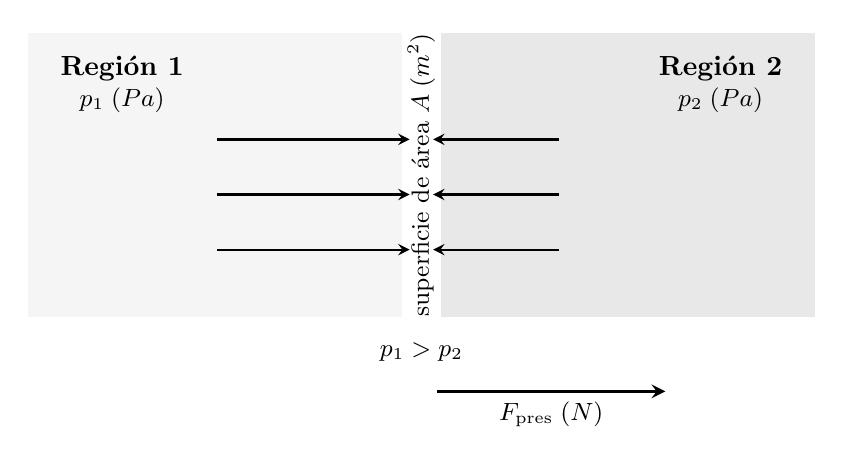
\begin{tikzpicture}[font=\small,>=stealth,x=1cm,y=1cm]
    \fill[black!4] (-5,-1.8) rectangle (0,1.8);
    \fill[black!9] (0,-1.8) rectangle (5,1.8);

    \draw[very thick] (0,-1.8) -- (0,1.8);
    \node[rotate=90,fill=white,inner sep=2pt] at (0,0)
        {superficie de área \(A\;(\text{m}^{2})\)};

    \node[font=\bfseries] at (-3.8,1.35) {Región 1};
    \node at (-3.8,0.95) {\(p_1\;(\text{Pa})\)};
    \node[font=\bfseries] at (3.8,1.35) {Región 2};
    \node at (3.8,0.95) {\(p_2\;(\text{Pa})\)};

    \foreach \y in {-0.95,-0.25,0.45}{
        \draw[->,thick] (-2.6,\y) -- (-0.15,\y);
        \draw[->,thick] (1.75,\y) -- (0.15,\y);
    }

    \node at (0,-2.25) {\(p_1>p_2\)};
    \draw[->,very thick] (0.2,-2.75) -- (3.1,-2.75)
        node[midway,below] {\(F_\mathrm{pres}\;(\text{N})\)};
\end{tikzpicture}

    \caption{Fuerza neta debida a una diferencia de presión uniforme sobre una
    superficie. Si \(p_1>p_2\), las contribuciones opuestas no se equilibran y
    la fuerza \(F_\mathrm{pres}=(p_1-p_2)A\) apunta hacia la región de menor
    presión. Esquema cualitativo de elaboración propia; no está dibujado a
    escala.}
    \label{fig:u2-fuerza-area}
\end{figure}

\subsubsection*{Ejemplo resuelto: fuerza sobre una superficie modelo}

Una superficie modelo tiene un área \(A=2{,}0\times10^{-4}\,\text{m}^{2}\). En un instante, la diferencia de presión entre sus lados es \(\Delta p=0{,}50\,\text{Pa}\). Bajo el supuesto de presión uniforme, la fuerza neta debida a la presión es:

\[
    F_\mathrm{pres}
    =(0{,}50\,\text{Pa})(2{,}0\times10^{-4}\,\text{m}^{2})
    =1{,}0\times10^{-4}\,\text{N}.
\]

El resultado describe una superficie ideal. No debe interpretarse como un valor universal de fuerza sobre la membrana timpánica: en una membrana real la presión puede variar con la posición y el movimiento está distribuido en toda su superficie.

\subsection{Tercera ley: fuerzas de interacción}
\label{sec:u2-tercera-ley}

Si un cuerpo \(A\) ejerce sobre un cuerpo \(B\) una fuerza \(\vec F_{A\rightarrow B}\), el cuerpo \(B\) ejerce simultáneamente sobre \(A\) una fuerza \(\vec F_{B\rightarrow A}\) de igual módulo y sentido opuesto:

\begin{equation}
    \vec F_{A\rightarrow B}=-\vec F_{B\rightarrow A}.
    \label{eq:u2-tercera-ley}
\end{equation}

Las dos fuerzas no se anulan entre sí porque actúan sobre cuerpos diferentes. Para estudiar la aceleración de \(B\), se suman las fuerzas que actúan sobre \(B\); la fuerza ejercida por \(B\) sobre \(A\) pertenece al diagrama de fuerzas de \(A\).

En el aire, elementos vecinos del medio ejercen fuerzas entre sí. Sin embargo, la tercera ley no basta para explicar la propagación del sonido. También se necesitan la compresibilidad del medio, los gradientes de presión y la inercia de sus partículas. La diferencia entre oscilación local y propagación se desarrollará en la Unidad~\ref{chap:unidad-3}.

\section{Masa, elasticidad y amortiguamiento}
\label{sec:u2-masa-resorte-amortiguador}

\subsection{Interpretación física}
\label{sec:u2-msa-interpretacion}

Un sistema mecánico sencillo puede representarse mediante tres propiedades:

\begin{description}
    \item[\textbf{Masa:}] caracteriza la inercia. Una masa mayor requiere una fuerza neta mayor para alcanzar la misma aceleración.
    \item[\textbf{Elasticidad:}] produce una fuerza restauradora cuando el sistema se separa de su posición de equilibrio.
    \item[\textbf{Amortiguamiento:}] representa mecanismos que se oponen al movimiento y convierten parte de la energía mecánica en energía interna.
\end{description}

Este modelo se denomina \textbf{sistema masa--resorte--amortiguador}. No supone que toda estructura biológica sea literalmente una masa unida a un resorte: concentra propiedades distribuidas en elementos ideales para facilitar el razonamiento.

La figura~\ref{fig:u2-masa-resorte-amortiguador} muestra la representación
unidimensional que se utilizará. El resorte y el amortiguador están conectados
en paralelo a la masa, por lo que ambos pueden ejercer fuerzas sobre ella
mientras actúa una fuerza externa.

\begin{figure}[htbp]
    \centering
    % Propósito: identificar los elementos ideales del modelo
% masa--resorte--amortiguador y las magnitudes asociadas.
% Origen: F_el=-kx, F_amort=-bv y F_ext-kx-bv=ma, ecuaciones
% \eqref{eq:u2-hooke}, \eqref{eq:u2-amortiguamiento} y \eqref{eq:u2-msa}.
% Esquema cualitativo, no a escala.
% Descripción accesible: una masa m puede desplazarse horizontalmente. Está
% conectada en paralelo a una pared mediante un resorte de rigidez k y un
% amortiguador de coeficiente b. Una fuerza externa F_ext apunta hacia el
% sentido positivo del desplazamiento x.
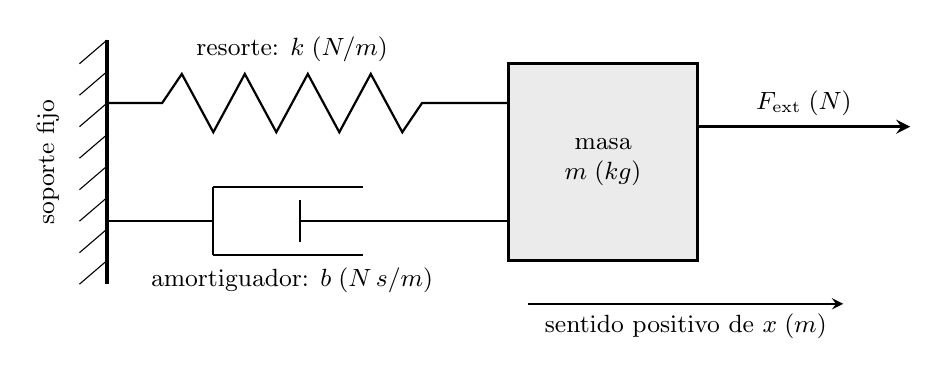
\begin{tikzpicture}[font=\small,>=stealth,x=1cm,y=1cm]
    % Pared fija.
    \draw[very thick] (0,-1.55) -- (0,1.55);
    \foreach \y in {-1.4,-1.0,...,1.4}{
        \draw (-0.35,\y-0.15) -- (0,\y+0.15);
    }
    \node[rotate=90] at (-0.75,0) {soporte fijo};

    % Resorte.
    \draw[thick] (0,0.75) -- (0.7,0.75)
        -- (0.95,1.12) -- (1.35,0.38)
        -- (1.75,1.12) -- (2.15,0.38)
        -- (2.55,1.12) -- (2.95,0.38)
        -- (3.35,1.12) -- (3.75,0.38)
        -- (4.0,0.75) -- (5.1,0.75);
    \node[above] at (2.35,1.15) {resorte: \(k\;(\text{N}/\text{m})\)};

    % Amortiguador viscoso ideal.
    \draw[thick] (0,-0.75) -- (1.35,-0.75);
    \draw[thick] (1.35,-1.18) -- (1.35,-0.32);
    \draw[thick] (1.35,-1.18) -- (3.25,-1.18);
    \draw[thick] (1.35,-0.32) -- (3.25,-0.32);
    \draw[thick] (2.45,-1.02) -- (2.45,-0.48);
    \draw[thick] (2.45,-0.75) -- (5.1,-0.75);
    \node[below] at (2.35,-1.22)
        {amortiguador: \(b\;(\text{N}\,\text{s}/\text{m})\)};

    % Masa y fuerza externa.
    \draw[very thick,fill=black!8] (5.1,-1.25) rectangle (7.5,1.25);
    \node[align=center] at (6.3,0)
        {masa\\\(m\;(\text{kg})\)};
    \draw[->,very thick] (7.5,0.45) -- (10.2,0.45)
        node[midway,above] {\(F_\mathrm{ext}\;(\text{N})\)};
    \draw[->,thick] (5.35,-1.8) -- (9.35,-1.8)
        node[midway,below] {sentido positivo de \(x\;(\text{m})\)};
\end{tikzpicture}

    \caption{Modelo ideal masa--resorte--amortiguador. La masa \(m\) representa
    la inercia, la rigidez \(k\) caracteriza la respuesta elástica y el
    coeficiente \(b\) representa el amortiguamiento viscoso lineal. El esquema
    es cualitativo y de elaboración propia; no representa la geometría literal
    de una estructura biológica.}
    \label{fig:u2-masa-resorte-amortiguador}
\end{figure}

\subsection{Modelo unidimensional}
\label{sec:u2-msa-modelo}

Sea \(x\) el desplazamiento respecto de la posición de equilibrio, medido en metros (\(\text{m}\)). La rigidez del resorte se representa mediante \(k\), medida en newtons por metro (\(\text{N}/\text{m}\)). En el modelo lineal, la fuerza elástica es:

\begin{equation}
    F_\mathrm{el}=-kx.
    \label{eq:u2-hooke}
\end{equation}

El signo negativo indica que la fuerza elástica apunta hacia la posición de equilibrio. Esta relación es una aproximación válida cuando el sistema trabaja dentro de un intervalo en el que fuerza y desplazamiento son aproximadamente proporcionales.

Sea \(v\) la velocidad del sistema, medida en metros por segundo (\(\text{m}/\text{s}\)). El coeficiente de amortiguamiento se representará mediante \(b\), medido en newton segundo por metro (\(\text{N}\,\text{s}/\text{m}\)). En un modelo de amortiguamiento viscoso lineal:

\begin{equation}
    F_\mathrm{amort}=-bv.
    \label{eq:u2-amortiguamiento}
\end{equation}

Si \(F_\mathrm{ext}\) es la fuerza externa aplicada, medida en newtons, la segunda ley permite escribir:

\begin{equation}
    F_\mathrm{ext}-kx-bv=ma.
    \label{eq:u2-msa}
\end{equation}

Cada término de la ecuación~\eqref{eq:u2-msa} tiene unidad de fuerza. La Unidad~\ref{chap:unidad-3} estudiará cómo evoluciona una oscilación con el tiempo. Por ahora interesa reconocer qué efecto representa cada término.

\subsection{Ejemplo resuelto: balance instantáneo de fuerzas}
\label{sec:u2-ejemplo-msa}

En un instante determinado, un sistema modelo tiene:

\begin{itemize}
    \item masa \(m=0{,}010\,\text{kg}\);
    \item rigidez \(k=20\,\text{N}/\text{m}\);
    \item coeficiente de amortiguamiento \(b=0{,}50\,\text{N}\,\text{s}/\text{m}\);
    \item desplazamiento \(x=0{,}0030\,\text{m}\);
    \item velocidad \(v=0{,}040\,\text{m}/\text{s}\);
    \item fuerza externa \(F_\mathrm{ext}=0{,}12\,\text{N}\).
\end{itemize}

Se adopta como positivo el sentido del desplazamiento y de la velocidad. La fuerza elástica y la fuerza de amortiguamiento apuntan en sentido opuesto:

\[
    F_\mathrm{el}
    =-(20\,\text{N}/\text{m})(0{,}0030\,\text{m})
    =-0{,}060\,\text{N},
\]

\[
    F_\mathrm{amort}
    =-(0{,}50\,\text{N}\,\text{s}/\text{m})(0{,}040\,\text{m}/\text{s})
    =-0{,}020\,\text{N}.
\]

La fuerza neta y la aceleración son:

\[
    F_\mathrm{neta}
    =0{,}12\,\text{N}-0{,}060\,\text{N}-0{,}020\,\text{N}
    =0{,}040\,\text{N},
\]

\[
    a=\frac{F_\mathrm{neta}}{m}
    =\frac{0{,}040\,\text{N}}{0{,}010\,\text{kg}}
    =4{,}0\,\text{m}/\text{s}^{2}.
\]

La aceleración es positiva en ese instante, pero esto no permite conocer por sí solo la velocidad o la posición en un instante posterior. Para ello sería necesario resolver la evolución temporal del sistema.

\subsection{Amortiguamiento y atenuación}
\label{sec:u2-amortiguamiento-atenuacion}

El amortiguamiento describe la disminución de una oscilación dentro de un sistema debido a mecanismos disipativos. La atenuación, en cambio, es una disminución de una magnitud o de un nivel durante una transmisión o propagación. Puede deberse a disipación, pero también a redistribución espacial, transmisión hacia otros medios o dispersión. Por lo tanto, no toda atenuación es causada por rozamiento ni toda disminución medida implica que la energía haya sido destruida.

\section{Trabajo, energía y disipación}
\label{sec:u2-energia}

\subsection{Trabajo y formas de energía mecánica}
\label{sec:u2-trabajo-energia}

Una fuerza puede transferir energía cuando produce un desplazamiento. En el caso sencillo de una fuerza constante, paralela al desplazamiento, sea \(F\) el módulo de la fuerza, medido en newtons, y sea \(d\) el desplazamiento, medido en metros. El trabajo mecánico \(W_\mathrm{trab}\), medido en joules (\(\text{J}\)), es:

\begin{equation}
    W_\mathrm{trab}=Fd.
    \label{eq:u2-trabajo}
\end{equation}

Un joule equivale a un newton metro: \(1\,\text{J}=1\,\text{N}\,\text{m}\).

Si un cuerpo de masa \(m\), medida en kilogramos, se mueve con rapidez \(v\), medida en metros por segundo, su energía cinética \(E_\mathrm{c}\), medida en joules, es:

\begin{equation}
    E_\mathrm{c}=\frac{1}{2}mv^{2}.
    \label{eq:u2-energia-cinetica}
\end{equation}

En un resorte lineal de rigidez \(k\), medida en newtons por metro, desplazado una distancia \(x\), medida en metros, la energía potencial elástica \(E_\mathrm{el}\), medida en joules, es:

\begin{equation}
    E_\mathrm{el}=\frac{1}{2}kx^{2}.
    \label{eq:u2-energia-elastica}
\end{equation}

En un sistema ideal sin amortiguamiento, la energía puede transformarse entre energía cinética y energía potencial elástica. En un sistema real, parte de la energía mecánica se transfiere a otras partes del entorno o se convierte de manera irreversible en energía interna.

\subsection{Conservación y pérdida de energía útil}
\label{sec:u2-conservacion-disipacion}

La conservación de la energía establece que la energía total de un sistema aislado permanece constante. Sin embargo, la energía disponible para producir un movimiento determinado puede disminuir. Para un balance didáctico durante un intervalo, se utilizarán las siguientes cantidades, todas medidas en joules:

\begin{itemize}
    \item \(E_\mathrm{entrada}\): energía que ingresa al sistema;
    \item \(\Delta E_\mathrm{mec}\): cambio de su energía mecánica almacenada;
    \item \(E_\mathrm{salida}\): energía transferida desde el sistema hacia otro;
    \item \(E_\mathrm{disipada}\): energía mecánica convertida en energía interna mediante procesos irreversibles.
\end{itemize}

Un balance posible es:

\begin{equation}
    E_\mathrm{entrada}
    =\Delta E_\mathrm{mec}
    +E_\mathrm{salida}
    +E_\mathrm{disipada}.
    \label{eq:u2-balance-energia}
\end{equation}

La expresión ``pérdida de energía'' debe interpretarse con cuidado. En muchos problemas significa pérdida de \emph{energía mecánica útil} para la función analizada, no desaparición de energía total. Una reflexión o una transmisión pueden reducir la energía recibida en un punto porque la redistribuyen; la disipación, en cambio, convierte energía mecánica organizada en energía interna.

\subsection{Ejemplo resuelto: balance de energía}
\label{sec:u2-ejemplo-energia}

Un sistema recibe \(E_\mathrm{entrada}=2{,}0\,\text{mJ}\). Al finalizar el intervalo, su energía mecánica aumentó \(\Delta E_\mathrm{mec}=1{,}3\,\text{mJ}\) y transfirió \(E_\mathrm{salida}=0{,}4\,\text{mJ}\) a otro sistema. Si no se consideran otras vías, la energía disipada es:

\[
    E_\mathrm{disipada}
    =2{,}0\,\text{mJ}-1{,}3\,\text{mJ}-0{,}4\,\text{mJ}
    =0{,}3\,\text{mJ}.
\]

La energía total se conserva. Lo que disminuye es la fracción de la energía de entrada que permanece como energía mecánica en el sistema o que se transfiere por la vía considerada útil.

\section{Temperatura, calor y entropía}
\label{sec:u2-termodinamica}

\subsection{Tres conceptos que no son equivalentes}
\label{sec:u2-temperatura-calor-interna}

La \textbf{temperatura} caracteriza el estado térmico de un sistema. Las temperaturas ambientales del libro se expresarán por defecto en grados Celsius (\(^{\circ}\text{C}\)). Cuando una ecuación requiera temperatura absoluta se utilizará \(T\), medida en kelvin (\(\text{K}\)).

La \textbf{energía interna}, que se representará mediante \(U\) y se medirá en joules (\(\text{J}\)), comprende formas microscópicas de energía asociadas al estado del sistema. No es sinónimo de temperatura: dos sistemas a la misma temperatura pueden poseer energías internas diferentes.

El \textbf{calor}, que se representará mediante \(Q\) y se medirá en joules, es energía transferida debido a una diferencia de temperatura. Un cuerpo no ``contiene calor'' como propiedad almacenada; posee energía interna y puede intercambiar energía mediante calor.

\subsection{Primera ley de la termodinámica}
\label{sec:u2-primera-ley-termodinamica}

Sea \(\Delta U\) el cambio de energía interna del sistema, medido en joules. Sea \(Q\) el calor recibido por el sistema y sea \(W_\mathrm{sobre}\) el trabajo realizado sobre él, ambos medidos en joules. Con esta convención de signos, la primera ley de la termodinámica se expresa como:

\begin{equation}
    \Delta U=Q+W_\mathrm{sobre}.
    \label{eq:u2-primera-ley-termo}
\end{equation}

Si el sistema recibe calor o si el entorno realiza trabajo sobre él, esos aportes pueden aumentar su energía interna. Una convención alternativa podría usar el trabajo realizado por el sistema; en ese caso cambiaría el signo del término de trabajo. La convención siempre debe declararse antes de calcular.

\subsection{Entropía e irreversibilidad}
\label{sec:u2-entropia}

La entropía \(S\) es una magnitud de estado termodinámica y se mide en joules por kelvin (\(\text{J}/\text{K}\)). En esta unidad se utilizará para reconocer la dirección de los procesos irreversibles. En un sistema total aislado, los procesos reales cumplen:

\begin{equation}
    \Delta S_\mathrm{total}\geq 0,
    \label{eq:u2-entropia}
\end{equation}

donde \(\Delta S_\mathrm{total}\) es el cambio de entropía total, medido en joules por kelvin. La igualdad corresponde al límite reversible ideal; una desigualdad estricta indica producción de entropía.

Describir la entropía únicamente como ``desorden'' resulta insuficiente: no permite calcularla ni distinguirla de la dispersión espacial de una onda. Los ecos y la reverberación son fenómenos de reflexión y persistencia temporal, no medidas de entropía. Cuando el rozamiento interno o la viscosidad convierten energía mecánica en energía interna, el proceso es irreversible y produce entropía.

\subsection{Compresión del aire y velocidad del sonido}
\label{sec:u2-temperatura-velocidad}

Una onda sonora en aire produce pequeñas compresiones y rarefacciones alrededor del estado de equilibrio. La compresión tiende a aumentar la presión y la temperatura locales; la expansión produce el cambio opuesto. En el modelo acústico lineal usual, estas variaciones son suficientemente rápidas y pequeñas como para aproximar cada ciclo local como un proceso adiabático, es decir, con intercambio de calor despreciable durante ese intervalo~\cite{xiangBlauert2021}.

La velocidad de propagación no es la velocidad local de las partículas del aire. Se representará mediante \(c\) y se medirá en metros por segundo (\(\text{m}/\text{s}\)). Para un gas ideal bajo el modelo adiabático, sean:

\begin{itemize}
    \item \(\gamma\), la razón de capacidades caloríficas, sin unidad;
    \item \(R\), la constante molar de los gases. Su unidad es el joule por mol kelvin (\(\text{J}\,\text{mol}^{-1}\,\text{K}^{-1}\));
    \item \(T\), la temperatura absoluta, medida en kelvin;
    \item \(M\), la masa molar del gas, medida en kilogramos por mol (\(\text{kg}/\text{mol}\)).
\end{itemize}

Bajo esas hipótesis, la velocidad de propagación se modela mediante~\cite{cramer1993,xiangBlauert2021}

\begin{equation}
    c=\sqrt{\frac{\gamma RT}{M}}.
    \label{eq:u2-velocidad-gas}
\end{equation}

Si la composición del gas se mantiene constante, la ecuación~\eqref{eq:u2-velocidad-gas} muestra que \(c\) aumenta con la raíz cuadrada de la temperatura absoluta. La densidad por sí sola no determina la velocidad: también importa la respuesta elástica del medio.

Para aire seco y temperaturas cercanas a las ambientales puede utilizarse, como aproximación didáctica~\cite{cramer1993,xiangBlauert2021},

\begin{equation}
    c\approx
    331\,\text{m}/\text{s}
    +\left(0{,}6\,\frac{\text{m}/\text{s}}{^{\circ}\text{C}}\right)\vartheta,
    \label{eq:u2-velocidad-temperatura}
\end{equation}

donde \(\vartheta\) es la temperatura ambiental expresada en grados Celsius.
Esta aproximación no incluye por separado los efectos de composición, humedad
o presión y no debe extrapolarse fuera del intervalo para el que se valide.

\subsubsection*{Ejemplo resuelto: cambio de velocidad con la temperatura}

Aplicando la aproximación de la ecuación~\eqref{eq:u2-velocidad-temperatura},
para \(\vartheta=20\,^{\circ}\text{C}\):

\[
    c\approx331\,\text{m}/\text{s}
    +\left(0{,}6\,\frac{\text{m}/\text{s}}{^{\circ}\text{C}}\right)
    (20\,^{\circ}\text{C})
    =343\,\text{m}/\text{s}.
\]

Para \(\vartheta=30\,^{\circ}\text{C}\):

\[
    c\approx349\,\text{m}/\text{s}.
\]

Según este modelo, el aumento de \(10\,^{\circ}\text{C}\) produce un aumento aproximado de \(6\,\text{m}/\text{s}\). Esto no significa que un tono de frecuencia fija adquiera automáticamente mayor altura tonal. La velocidad de propagación es una magnitud física; la altura tonal o \emph{pitch} es un atributo perceptual. Si la frecuencia de la fuente se mantiene, el cambio de velocidad modifica principalmente la longitud de onda, relación que se formalizará en la Unidad~\ref{chap:unidad-3}.

La figura~\ref{fig:u2-velocidad-temperatura} permite leer esa tendencia dentro
del intervalo usado en el ejemplo. Los puntos pertenecen al modelo de la
ecuación~\eqref{eq:u2-velocidad-temperatura}; no son mediciones experimentales.

\begin{figure}[ht]
    \centering
    % Propósito: enseñar a leer la tendencia de la aproximación lineal de la
% velocidad del sonido con la temperatura ambiental.
% Origen: c=(331+0,6 theta) m/s, ecuación
% \eqref{eq:u2-velocidad-temperatura}. Los puntos son valores calculados del
% modelo, no mediciones. Intervalo representado: 0 a 30 grados Celsius.
% Descripción accesible: un gráfico cartesiano muestra la temperatura entre
% 0 y 30 grados Celsius en el eje horizontal y la velocidad entre 325 y
% 355 metros por segundo en el eje vertical. Una recta ascendente pasa por
% los puntos 331, 337, 343 y 349 metros por segundo para 0, 10, 20 y 30 grados
% Celsius, respectivamente.
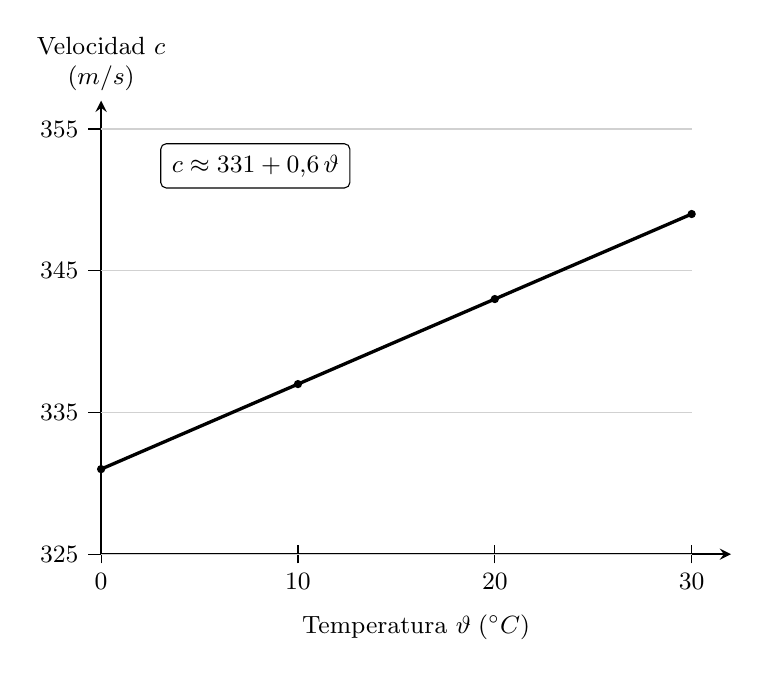
\begin{tikzpicture}[font=\small,>=stealth,x=0.25cm,y=0.18cm]
    % La coordenada vertical representa c-325 para mantener legibles las
    % variaciones dentro del intervalo declarado.
    \draw[->,thick] (0,0) -- (32,0);
    \node[below] at (16,-3.6)
        {Temperatura \(\vartheta\;({}^{\circ}\text{C})\)};
    \draw[->,thick] (0,0) -- (0,32);
    \node[above,align=center] at (0,32)
        {Velocidad \(c\)\\\((\text{m}/\text{s})\)};

    \foreach \temp in {0,10,20,30}{
        \draw (\temp,-0.65) -- (\temp,0.65);
        \node[below] at (\temp,-0.65) {\temp};
    }
    \foreach \vel in {325,335,345,355}{
        \pgfmathsetmacro{\posy}{\vel-325}
        \draw (-0.65,\posy) -- (0.65,\posy);
        \node[left] at (-0.65,\posy) {\vel};
        \draw[black!18] (0,\posy) -- (30,\posy);
    }

    \draw[very thick] (0,6) -- (30,24);
    \foreach \temp/\vel in {0/331,10/337,20/343,30/349}{
        \pgfmathsetmacro{\posy}{\vel-325}
        \fill (\temp,\posy) circle (1.5pt);
    }

    \node[
        draw,
        fill=white,
        rounded corners=2pt,
        inner sep=4pt,
        anchor=north west
    ] at (3,29)
        {\(c\approx331+0{,}6\,\vartheta\)};
\end{tikzpicture}

    \caption{Velocidad de propagación calculada con la aproximación lineal
    \(c\approx331+0{,}6\vartheta\), para
    \(0\,^{\circ}\text{C}\leq\vartheta\leq
    30\,^{\circ}\text{C}\). La escala vertical se limita al intervalo
    \(325\)--\(355\,\text{m}/\text{s}\) para hacer visible la variación. Los
    puntos son resultados teóricos, no datos medidos. Elaboración propia a
    partir de la ecuación~\eqref{eq:u2-velocidad-temperatura}.}
    \label{fig:u2-velocidad-temperatura}
\end{figure}

\section{Relación con Fonoaudiología}
\label{sec:u2-fonoaudiologia}

Los modelos de esta unidad permiten organizar aplicaciones posteriores sin reemplazar la descripción anatómica o clínica:

\begin{description}
    \item[\textbf{Membrana timpánica:}] una diferencia de presión puede ejercer una fuerza sobre su superficie. Su respuesta mecánica puede analizarse cualitativamente mediante inercia, elasticidad y amortiguamiento, sin reducir la membrana real a una masa puntual.

    \item[\textbf{Cadena osicular:}] el oído medio funciona como un sistema mecánico pasivo que contribuye a la adaptación entre la impedancia del aire y la del oído interno. Puede transformar las relaciones entre presión, fuerza, velocidad y desplazamiento, pero no crea energía~\cite{ugarteburu2022}. Su mecánica se desarrollará en una unidad posterior.

    \item[\textbf{Vibrador óseo:}] un vibrador óseo aplica una fuerza variable al cráneo y pone en movimiento un sistema formado por el transductor, el punto de contacto y las estructuras de la cabeza. La audición por vía ósea resulta de varios mecanismos y no de una única onda que recorra el hueso~\cite{stenfeltGoode2005}. Estos mecanismos se estudiarán junto con el sistema auditivo.

    \item[\textbf{Disipación en tejidos:}] los tejidos biológicos presentan comportamiento viscoelástico: parte de la energía mecánica puede almacenarse de manera elástica y parte puede disiparse como energía interna~\cite{fung1981}. El modelo masa--resorte--amortiguador permite representar esta diferencia de manera introductoria.

    \item[\textbf{Propagación en aire:}] la compresibilidad y la inercia del aire permiten la propagación, mientras que su estado termodinámico influye en la velocidad. La absorción atmosférica, los gradientes y la propagación en exteriores se tratarán en la unidad correspondiente.
\end{description}

La figura~\ref{fig:u2-balance-energia-auditiva} organiza la transferencia de
energía a lo largo de una vía mecánica simplificada. Las salidas inferiores
recuerdan que una reducción de energía en la vía principal puede corresponder a
almacenamiento, transferencia hacia otra vía o disipación; no implica que la
energía desaparezca.

\begin{figure}[ht]
    \centering
    % Propósito: mostrar que la cadena auditiva pasiva transfiere y transforma
% energía, mientras parte puede almacenarse, salir de la vía o disiparse, sin
% creación de energía.
% Origen: balance E_entrada=Delta E_mec+E_salida+E_disipada, ecuación
% \eqref{eq:u2-balance-energia}, aplicado cualitativamente a la relación con
% Fonoaudiología. No representa eficiencias ni datos anatómicos.
% Descripción accesible: la energía mecánica de una perturbación en el aire
% llega a la membrana timpánica, pasa a la cadena osicular y se transfiere hacia
% el oído interno. Desde la membrana y la cadena salen flechas hacia una caja de
% energía interna u otras vías, que representan almacenamiento, transferencia
% fuera de la vía principal y disipación. Ninguna etapa crea energía.
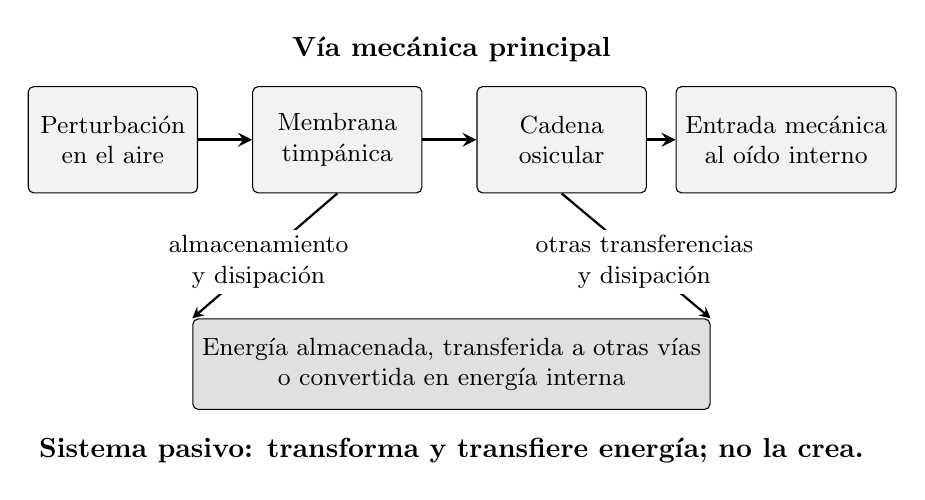
\begin{tikzpicture}[
    font=\small,
    >=stealth,
    bloque/.style={
        draw,
        rounded corners=2pt,
        minimum width=2.15cm,
        minimum height=1.35cm,
        align=center,
        fill=black!5
    }
]
    \node[bloque] (aire) at (0,0)
        {Perturbación\\en el aire};
    \node[bloque] (membrana) at (2.85,0)
        {Membrana\\timpánica};
    \node[bloque] (osiculos) at (5.7,0)
        {Cadena\\osicular};
    \node[bloque] (salida) at (8.55,0)
        {Entrada mecánica\\al oído interno};

    \node[font=\bfseries] at (4.3,1.15) {Vía mecánica principal};
    \draw[->,very thick] (aire.east) -- (membrana.west);
    \draw[->,very thick] (membrana.east) -- (osiculos.west);
    \draw[->,very thick] (osiculos.east) -- (salida.west);

    \node[
        draw,
        rounded corners=2pt,
        minimum width=5.8cm,
        minimum height=1.15cm,
        align=center,
        fill=black!12
    ] (otras) at (4.3,-2.85)
        {Energía almacenada, transferida a otras vías\\
        o convertida en energía interna};

    \draw[->,thick] (membrana.south) -- (otras.north west);
    \draw[->,thick] (osiculos.south) -- (otras.north east);
    \node[fill=white,align=center,inner sep=2pt] at (1.85,-1.55)
        {almacenamiento\\y disipación};
    \node[fill=white,align=center,inner sep=2pt] at (6.75,-1.55)
        {otras transferencias\\y disipación};

    \node[font=\bfseries] at (4.3,-3.95)
        {Sistema pasivo: transforma y transfiere energía; no la crea.};
\end{tikzpicture}

    \caption{Ruta conceptual de la energía mecánica desde el aire hacia el oído
    interno a través de la membrana timpánica y la cadena osicular. El diagrama
    distingue la transferencia por la vía principal de otras transferencias,
    del almacenamiento y de la disipación. Es un balance cualitativo de
    elaboración propia: no representa eficiencias ni implica creación de
    energía en ninguna etapa.}
    \label{fig:u2-balance-energia-auditiva}
\end{figure}

Estas conexiones son físicas. No permiten por sí solas obtener un diagnóstico, predecir una sensación sonora ni establecer un resultado audiométrico.

\section{Errores frecuentes}
\label{sec:u2-errores}

\begin{itemize}
    \item \textbf{Confundir presión con fuerza.} La presión se mide en pascales; la fuerza se mide en newtons. Para relacionarlas se necesita un área y una distribución de presión.
    \item \textbf{Atribuir el retorno al equilibrio a la primera ley.} El retorno requiere una fuerza restauradora; la reducción progresiva de la oscilación requiere amortiguamiento.
    \item \textbf{Usar \(F=ma\) con una sola fuerza.} La aceleración depende de la fuerza neta, no necesariamente de una fuerza individual.
    \item \textbf{Hacer actuar acción y reacción sobre el mismo cuerpo.} Las fuerzas de la tercera ley actúan sobre cuerpos diferentes.
    \item \textbf{Afirmar que el oído medio crea energía.} Un sistema pasivo puede transformar presión, fuerza, velocidad o desplazamiento sin aumentar la energía total.
    \item \textbf{Interpretar disipación como destrucción de energía.} La disipación convierte energía mecánica en energía interna; la energía total se conserva.
    \item \textbf{Definir calor como energía almacenada.} El calor es una forma de transferencia; la energía almacenada en el estado microscópico es energía interna.
    \item \textbf{Usar entropía como sinónimo de eco o desorden cotidiano.} La entropía es una magnitud termodinámica y los ecos se explican mediante reflexión.
    \item \textbf{Generalizar los efectos atmosféricos.} Temperatura, composición, humedad y presión no deben reemplazarse por una regla única sin condiciones.
    \item \textbf{Confundir velocidad de propagación con altura tonal.} Una es una magnitud física del sistema fuente--medio; la otra es un atributo perceptual.
\end{itemize}

\section{Síntesis}
\label{sec:u2-sintesis}

Las leyes de Newton relacionan interacciones y cambios de movimiento. La primera ley describe el caso de fuerza neta nula; la segunda vincula fuerza neta, masa y aceleración; la tercera identifica pares de fuerzas que actúan sobre cuerpos diferentes. Una diferencia de presión puede originar una fuerza sobre una superficie, pero presión y fuerza conservan unidades y significados distintos.

El modelo masa--resorte--amortiguador reúne inercia, elasticidad y disipación. La energía puede transformarse entre formas cinética y elástica, transferirse hacia otros sistemas o convertirse de manera irreversible en energía interna. La pérdida de energía mecánica útil no implica desaparición de energía total.

La temperatura, el calor y la energía interna no son equivalentes. La primera ley de la termodinámica establece un balance entre energía interna, calor y trabajo; la entropía permite reconocer la irreversibilidad. En un gas, la velocidad de propagación depende de sus propiedades termodinámicas. Esta velocidad física no debe confundirse con la velocidad local de las partículas ni con una cualidad perceptual.

\section{Ejercicios de autoevaluación}
\label{sec:u2-ejercicios}

La secuencia comienza con interpretación conceptual y gráfica, continúa con
cálculos guiados y autónomos, y termina con aplicaciones, distractores
razonables y una situación integradora. En los ejercicios numéricos se debe
escribir la ecuación utilizada, conservar las unidades durante el cálculo,
redondear solo el resultado final e interpretar su significado físico.

\subsection*{Preguntas conceptuales}

\begin{enumerate}[label=\textbf{C\arabic*.},leftmargin=*]
    \item Una estructura se mueve con velocidad constante. ¿Es obligatorio que
    no actúe ninguna fuerza sobre ella? Indique qué condición debe cumplir la
    fuerza neta.

    \item Compare dos sistemas sometidos a la misma fuerza neta. El sistema
    \(A\) tiene mayor masa que el sistema \(B\). ¿Cuál adquiere mayor
    aceleración? Relacione la respuesta con la inercia.

    \item Explique por qué la elasticidad, y no la primera ley de Newton,
    permite que una membrana desplazada tienda a volver al equilibrio. Indique
    además qué función cumple el amortiguamiento.

    \item Identifique los cuerpos sobre los que actúa cada fuerza en el par
    acción--reacción formado por una membrana y el aire que la empuja. Explique
    por qué esas fuerzas no se cancelan en el diagrama de un solo cuerpo.

    \item Compare amortiguamiento, atenuación y disipación. ¿Por qué una
    disminución de amplitud observada durante una transmisión no demuestra, por
    sí sola, que toda la energía se haya disipado por rozamiento?

    \item Distinga temperatura, calor, energía interna y entropía mediante una
    oración para cada concepto. Incluya la unidad de energía interna y la de
    entropía.

    \item Explique qué significa ``pérdida de energía mecánica útil'' sin
    violar la conservación de la energía. Aplique la respuesta a un sistema
    mecánico pasivo que modifica presión, fuerza, velocidad o desplazamiento.

    \item Si cambia la velocidad de propagación del sonido en aire mientras la
    frecuencia de la fuente permanece fija, ¿puede concluirse que cambia en la
    misma proporción la altura tonal percibida? Distinga la magnitud física del
    atributo perceptual.
\end{enumerate}

\subsection*{Identificación e interpretación de figuras y gráficos}

\begin{enumerate}[label=\textbf{R\arabic*.},leftmargin=*]
    \item Observe la figura~\ref{fig:u2-fuerza-area}.
    \begin{enumerate}[label=\alph*)]
        \item Identifique las dos contribuciones de presión y el sentido de la
        fuerza neta cuando \(p_1>p_2\).
        \item ¿Qué ocurriría con la fuerza neta debida a la presión si
        \(p_1=p_2\)?
        \item Explique por qué \(p_1\), \(p_2\) y \(F_\mathrm{pres}\) no pueden
        expresarse con la misma unidad.
    \end{enumerate}

    \item Observe la figura~\ref{fig:u2-masa-resorte-amortiguador}.
    \begin{enumerate}[label=\alph*)]
        \item Asocie masa, resorte y amortiguador con inercia, elasticidad y
        disipación, respectivamente.
        \item La figura fija hacia la derecha el sentido positivo de \(x\). Si
        en un instante \(x>0\) y \(v>0\), indique el sentido de
        \(F_\mathrm{el}\) y \(F_\mathrm{amort}\).
        \item ¿Qué limitación tendría interpretar el dibujo como una
        representación anatómica literal de la membrana timpánica?
    \end{enumerate}

    \item Observe la figura~\ref{fig:u2-velocidad-temperatura}.
    \begin{enumerate}[label=\alph*)]
        \item Identifique la magnitud y la unidad de cada eje.
        \item Lea aproximadamente \(c\) para
        \(\vartheta=0\,^{\circ}\text{C}\) y
        \(\vartheta=30\,^{\circ}\text{C}\).
        \item Determine cuánto aumenta \(c\) por cada incremento de
        \(10\,^{\circ}\text{C}\) dentro del intervalo representado.
        \item ¿Los puntos son mediciones o resultados del modelo? ¿Permite el
        gráfico concluir que aumenta la altura tonal percibida?
    \end{enumerate}

    \item Observe la figura~\ref{fig:u2-balance-energia-auditiva}.
    \begin{enumerate}[label=\alph*)]
        \item Identifique la vía mecánica principal y dos destinos posibles de
        la energía fuera de esa vía.
        \item Distinga almacenamiento, transferencia y disipación en el
        diagrama.
        \item Explique por qué la figura no permite calcular una eficiencia ni
        afirmar que la cadena osicular crea energía.
    \end{enumerate}
\end{enumerate}

\subsection*{Ejercicios numéricos guiados}

\begin{enumerate}[label=\textbf{NG\arabic*.},leftmargin=*]
    \item Una superficie modelo de área
    \(A=3{,}0\times10^{-4}\,\text{m}^{2}\) está sometida a una diferencia de
    presión uniforme \(\Delta p=0{,}40\,\text{Pa}\).
    \begin{enumerate}[label=\alph*)]
        \item Escriba la ecuación que relaciona diferencia de presión, área y
        fuerza.
        \item Sustituya los datos y compruebe que
        \(\text{Pa}\,\text{m}^{2}=\text{N}\).
        \item Calcule \(F_\mathrm{pres}\) con dos cifras significativas e
        indique su sentido respecto de la región de menor presión.
    \end{enumerate}

    \item En un instante, un sistema masa--resorte--amortiguador tiene los
    siguientes datos:
    \[
        \begin{aligned}
            m &= 0{,}020\,\text{kg},&
            k &= 25\,\text{N}/\text{m},\\
            b &= 0{,}40\,\text{N}\,\text{s}/\text{m},&
            x &= 0{,}0020\,\text{m},\\
            v &= 0{,}030\,\text{m}/\text{s},&
            F_\mathrm{ext} &= 0{,}090\,\text{N}.
        \end{aligned}
    \]
    El sentido de \(x\) y \(v\) es positivo.
    \begin{enumerate}[label=\alph*)]
        \item Calcule \(F_\mathrm{el}=-kx\).
        \item Calcule \(F_\mathrm{amort}=-bv\).
        \item Determine la fuerza neta mediante la
        ecuación~\eqref{eq:u2-msa}.
        \item Calcule la aceleración e interprete su signo.
    \end{enumerate}

    \item Un sistema recibe \(E_\mathrm{entrada}=2{,}0\,\text{mJ}\), aumenta su
    energía mecánica en
    \(\Delta E_\mathrm{mec}=1{,}2\,\text{mJ}\) y transfiere
    \(E_\mathrm{salida}=0{,}5\,\text{mJ}\) hacia otro sistema. No se consideran
    otras vías.
    \begin{enumerate}[label=\alph*)]
        \item Despeje \(E_\mathrm{disipada}\) del
        balance~\eqref{eq:u2-balance-energia}.
        \item Calcule su valor.
        \item Explique por qué el resultado no representa energía destruida.
    \end{enumerate}

    \item Un sistema transfiere \(3{,}0\,\text{J}\) de energía hacia el entorno
    mediante calor, mientras el entorno realiza sobre él un trabajo de
    \(2{,}0\,\text{J}\). Use la convención de la
    ecuación~\eqref{eq:u2-primera-ley-termo}.
    \begin{enumerate}[label=\alph*)]
        \item Asigne los signos de \(Q\) y \(W_\mathrm{sobre}\).
        \item Calcule \(\Delta U\).
        \item Indique si la energía interna aumenta o disminuye.
    \end{enumerate}
\end{enumerate}

\subsection*{Ejercicios numéricos autónomos}

\begin{enumerate}[label=\textbf{NA\arabic*.},leftmargin=*]
    \item Un resorte lineal tiene una rigidez
    \(k=30\,\text{N}/\text{m}\) y se desplaza
    \(x=0{,}0040\,\text{m}\). Calcule:
    \begin{enumerate}[label=\alph*)]
        \item el módulo de la fuerza elástica;
        \item la energía potencial elástica almacenada.
    \end{enumerate}

    \item Sobre una masa \(m=0{,}015\,\text{kg}\) actúan, en la dirección
    analizada, \(F_\mathrm{ext}=0{,}080\,\text{N}\),
    \(F_\mathrm{el}=-0{,}030\,\text{N}\) y
    \(F_\mathrm{amort}=-0{,}020\,\text{N}\). Calcule la fuerza neta y la
    aceleración.

    \item Un sistema recibe \(E_\mathrm{entrada}=3{,}6\,\text{mJ}\), almacena
    \(\Delta E_\mathrm{mec}=1{,}4\,\text{mJ}\) y transfiere
    \(E_\mathrm{salida}=1{,}5\,\text{mJ}\). Si no existen otras vías, calcule
    \(E_\mathrm{disipada}\).

    \item Para un proceso se informa
    \(Q=4{,}5\,\text{J}\) y
    \(W_\mathrm{sobre}=-1{,}5\,\text{J}\). Calcule \(\Delta U\) con la
    convención de la ecuación~\eqref{eq:u2-primera-ley-termo} e interprete el
    signo.

    \item Aplique la ecuación~\eqref{eq:u2-velocidad-temperatura} a dos estados
    uniformes de aire seco:
    \(\vartheta_1=5\,^{\circ}\text{C}\) y
    \(\vartheta_2=25\,^{\circ}\text{C}\).
    \begin{enumerate}[label=\alph*)]
        \item Calcule \(c_1\) y \(c_2\).
        \item Una señal recorre en cada estado una distancia
        \(d=100{,}0\,\text{m}\). Calcule los tiempos de propagación
        \(t_1=d/c_1\) y \(t_2=d/c_2\).
        \item Determine la diferencia entre ambos tiempos en milisegundos.
    \end{enumerate}
\end{enumerate}

\subsection*{Aplicaciones en Fonoaudiología}

\begin{enumerate}[label=\textbf{F\arabic*.},leftmargin=*]
    \item Para construir un modelo introductorio de la membrana timpánica se
    proponen masa, resorte y amortiguador. Indique qué propiedad física
    representa cada elemento, qué mecanismo permite el retorno al equilibrio y
    una limitación del modelo.

    \item Un vibrador óseo y la cabeza ejercen fuerzas entre sí. Identifique el
    par de fuerzas que satisface la tercera ley y explique por qué esas fuerzas
    no se cancelan al analizar solamente la cabeza.

    \item Una persona observa que la cadena osicular puede aumentar una presión
    mecánica y concluye que ``los huesecillos crean energía''. Corrija la
    conclusión mediante conservación, transferencia y disipación de energía.

    \item En un tejido se observa que una vibración disminuye a medida que
    avanza. Explique por qué esa observación no permite atribuir toda la
    atenuación al rozamiento. Mencione al menos otra posibilidad presentada en
    la unidad.

    \item Un mismo transductor emite una señal de frecuencia fija en dos
    estados uniformes del aire con temperaturas diferentes. Indique qué
    magnitud del medio cambia según el modelo de esta unidad y por qué ese
    cambio no equivale, por sí solo, a una modificación de la altura tonal
    percibida.
\end{enumerate}

\subsection*{Errores frecuentes y distractores}

\begin{enumerate}[label=\textbf{D\arabic*.},leftmargin=*]
    \item Para obtener una fuerza a partir de una diferencia de presión
    \(\Delta p\), medida en pascales, y un área \(A\), medida en metros
    cuadrados, se proponen:
    \[
        F_1=\Delta p\,A,
        \qquad
        F_2=\frac{\Delta p}{A},
        \qquad
        F_3=\frac{A}{\Delta p}.
    \]
    Seleccione la expresión físicamente coherente y descarte las otras mediante
    análisis dimensional.

    \item Para los datos del ejercicio \textbf{NG2}, se proponen como
    aceleración \(4{,}5\,\text{m}/\text{s}^{2}\),
    \(1{,}4\,\text{m}/\text{s}^{2}\) y
    \(7{,}6\,\text{m}/\text{s}^{2}\). Identifique el resultado correcto y
    explique qué fuerzas fueron omitidas o sumadas con signo incorrecto en los
    otros dos.

    \item Un balance informa
    \(E_\mathrm{entrada}=1{,}0\,\text{mJ}\),
    \(\Delta E_\mathrm{mec}=0{,}8\,\text{mJ}\) y
    \(E_\mathrm{salida}=0{,}5\,\text{mJ}\), sin otras entradas. Compruebe si
    esos datos son compatibles con
    \(E_\mathrm{disipada}\geq0\). Si no lo son, identifique la contradicción.

    \item Indique cuáles afirmaciones son correctas y corrija las restantes:
    \begin{enumerate}[label=\alph*)]
        \item ``si un cuerpo está en reposo, no actúa ninguna fuerza sobre él'';
        \item ``acción y reacción se cancelan porque actúan sobre el mismo
        cuerpo'';
        \item ``toda atenuación es causada por fricción'';
        \item ``la entropía es simplemente desorden'';
        \item ``si aumenta la temperatura del aire, necesariamente aumenta la
        altura tonal de una fuente de frecuencia fija'';
        \item ``un sistema auditivo pasivo puede transformar variables
        mecánicas sin crear energía''.
    \end{enumerate}
\end{enumerate}

\subsection*{Pregunta integradora}

\begin{enumerate}[label=\textbf{I\arabic*.},leftmargin=*]
    \item Se construye un sistema ideal para organizar una descripción
    introductoria de una superficie flexible. Los parámetros no representan
    valores anatómicos de una membrana timpánica. La superficie tiene
    \(A=2{,}0\times10^{-4}\,\text{m}^{2}\) y está sometida a
    \(\Delta p=0{,}50\,\text{Pa}\). La fuerza debida a la presión se toma como
    \(F_\mathrm{ext}\). En un instante, el modelo tiene
    \(m=2{,}0\times10^{-4}\,\text{kg}\),
    \(k=2{,}0\times10^{-2}\,\text{N}/\text{m}\),
    \(b=1{,}0\times10^{-3}\,\text{N}\,\text{s}/\text{m}\),
    \(x=2{,}0\times10^{-3}\,\text{m}\) y
    \(v=2{,}0\times10^{-2}\,\text{m}/\text{s}\), con \(x\) y \(v\) positivos.
    Durante otro intervalo del mismo modelo se adoptan
    \(E_\mathrm{entrada}=0{,}80\,\text{mJ}\),
    \(\Delta E_\mathrm{mec}=0{,}45\,\text{mJ}\) y
    \(E_\mathrm{salida}=0{,}20\,\text{mJ}\). El aire se encuentra a
    \(\vartheta=20\,^{\circ}\text{C}\).
    \begin{enumerate}[label=\alph*)]
        \item Calcule \(F_\mathrm{ext}=\Delta p\,A\).
        \item Calcule \(F_\mathrm{el}\), \(F_\mathrm{amort}\), la fuerza neta y
        la aceleración instantánea.
        \item Indique qué término favorece el retorno al equilibrio y cuál
        representa disipación.
        \item Calcule \(E_\mathrm{disipada}\) en el intervalo energético.
        \item Calcule la velocidad de propagación aproximada en el aire.
        \item Explique por qué ni el balance mecánico ni el energético permiten
        afirmar que una cadena osicular crea energía.
        \item Señale dos limitaciones del sistema ideal y explique por qué los
        resultados no constituyen una conclusión clínica ni predicen una
        sensación sonora.
    \end{enumerate}
\end{enumerate}

\section{Soluciones de los ejercicios}
\label{sec:u2-soluciones}

\subsection*{Preguntas conceptuales}

\begin{enumerate}[label=\textbf{C\arabic*.},leftmargin=*]
    \item No. Pueden actuar varias fuerzas cuya suma sea nula. La velocidad
    permanece constante cuando \(F_\mathrm{neta}=0\).

    \item De \(a=F_\mathrm{neta}/m\) se obtiene que, a igual fuerza neta, el
    sistema de menor masa adquiere mayor aceleración. Por lo tanto, \(B\)
    acelera más que \(A\); la mayor masa de \(A\) representa mayor inercia.

    \item La primera ley describe el caso de fuerza neta nula. El retorno
    requiere una fuerza elástica dirigida hacia la posición de equilibrio. El
    amortiguamiento se opone al movimiento y reduce progresivamente la energía
    mecánica de la oscilación.

    \item El aire ejerce una fuerza sobre la membrana y la membrana ejerce una
    fuerza igual y opuesta sobre el aire. Cada fuerza actúa sobre un cuerpo
    diferente; al analizar solo la membrana se incluye la primera, no la fuerza
    que actúa sobre el aire.

    \item El amortiguamiento reduce una oscilación dentro de un sistema; la
    atenuación describe una disminución durante una transmisión o propagación;
    la disipación convierte energía mecánica en energía interna. Una atenuación
    también puede deberse a redistribución espacial o transferencia hacia otra
    vía, por lo que no demuestra por sí sola que haya rozamiento.

    \item La temperatura caracteriza el estado térmico. El calor es energía
    transferida por diferencia de temperatura. La energía interna pertenece al
    estado microscópico del sistema y se mide en joules
    (\(\text{J}\)). La entropía es una magnitud de estado que permite
    caracterizar la irreversibilidad y se mide en joules por kelvin
    (\(\text{J}/\text{K}\)).

    \item Significa que disminuye la energía disponible en la forma o vía que
    interesa. Un sistema pasivo puede modificar las relaciones entre presión,
    fuerza, velocidad y desplazamiento mientras transfiere, almacena o disipa
    energía, pero no crea energía total.

    \item No. La velocidad de propagación es una magnitud física del medio. La
    altura tonal es un atributo perceptual y no puede deducirse únicamente a
    partir de un cambio de velocidad si la frecuencia de la fuente permanece
    fija.
\end{enumerate}

\subsection*{Identificación e interpretación de figuras y gráficos}

\begin{enumerate}[label=\textbf{R\arabic*.},leftmargin=*]
    \item
    \begin{enumerate}[label=\alph*)]
        \item \(p_1\) ejerce una contribución hacia la derecha y \(p_2\) una
        contribución hacia la izquierda. Para \(p_1>p_2\), la fuerza neta
        apunta hacia la región 2.
        \item Si \(p_1=p_2\), entonces \(\Delta p=0\,\text{Pa}\) y la fuerza
        neta debida a esas presiones es \(0\,\text{N}\).
        \item \(p_1\) y \(p_2\) son presiones y se miden en pascales; la fuerza
        se mide en newtons. El área permite relacionarlas mediante
        \(F_\mathrm{pres}=\Delta p\,A\).
    \end{enumerate}

    \item
    \begin{enumerate}[label=\alph*)]
        \item La masa representa inercia; el resorte, elasticidad; el
        amortiguador, disipación dependiente del movimiento.
        \item Si \(x>0\), \(F_\mathrm{el}=-kx<0\). Si \(v>0\),
        \(F_\mathrm{amort}=-bv<0\). Ambas fuerzas apuntan hacia el sentido
        negativo en ese instante.
        \item La membrana real posee geometría, masa, rigidez y amortiguamiento
        distribuidos; no es una masa rígida conectada literalmente a dos
        elementos concentrados.
    \end{enumerate}

    \item
    \begin{enumerate}[label=\alph*)]
        \item El eje horizontal representa \(\vartheta\) en grados Celsius
        (\(^{\circ}\text{C}\)); el vertical representa \(c\) en metros por
        segundo (\(\text{m}/\text{s}\)).
        \item Se leen aproximadamente \(331\,\text{m}/\text{s}\) para
        \(0\,^{\circ}\text{C}\) y \(349\,\text{m}/\text{s}\) para
        \(30\,^{\circ}\text{C}\).
        \item El incremento es aproximadamente
        \(6\,\text{m}/\text{s}\) por cada \(10\,^{\circ}\text{C}\).
        \item Son resultados de la aproximación teórica, no mediciones. El
        gráfico representa una magnitud física del medio y no permite concluir
        que aumente la altura tonal percibida.
    \end{enumerate}

    \item
    \begin{enumerate}[label=\alph*)]
        \item La vía principal va desde la perturbación en el aire hasta la
        entrada mecánica al oído interno, pasando por membrana y cadena
        osicular. Fuera de ella puede haber almacenamiento, transferencia hacia
        otras vías o conversión en energía interna.
        \item Almacenar conserva temporalmente energía mecánica. Transferirla la
        lleva a otro sistema o vía. Disiparla la convierte de manera
        irreversible en energía interna.
        \item El diagrama no contiene valores de entrada o salida, por lo que no
        permite calcular una eficiencia. Además, presenta un sistema pasivo que
        transfiere y transforma energía sin crearla.
    \end{enumerate}
\end{enumerate}

\subsection*{Ejercicios numéricos guiados}

\begin{enumerate}[label=\textbf{NG\arabic*.},leftmargin=*]
    \item Se utiliza la ecuación~\eqref{eq:u2-presion-fuerza}:
    \[
        F_\mathrm{pres}
        =\Delta p\,A
        =(0{,}40\,\text{Pa})(3{,}0\times10^{-4}\,\text{m}^{2})
        =1{,}2\times10^{-4}\,\text{N}.
    \]
    Las unidades cumplen
    \(\text{Pa}\,\text{m}^{2}
    =(\text{N}/\text{m}^{2})\text{m}^{2}
    =\text{N}\). La fuerza apunta hacia la región de menor presión.

    \item
    \[
        F_\mathrm{el}
        =-(25\,\text{N}/\text{m})(0{,}0020\,\text{m})
        =-0{,}050\,\text{N},
    \]
    \[
        F_\mathrm{amort}
        =-(0{,}40\,\text{N}\,\text{s}/\text{m})
        (0{,}030\,\text{m}/\text{s})
        =-0{,}012\,\text{N}.
    \]
    Por lo tanto:
    \[
        F_\mathrm{neta}
        =0{,}090\,\text{N}-0{,}050\,\text{N}-0{,}012\,\text{N}
        =0{,}028\,\text{N},
    \]
    \[
        a=\frac{0{,}028\,\text{N}}{0{,}020\,\text{kg}}
        =1{,}4\,\text{m}/\text{s}^{2}.
    \]
    La aceleración es positiva en el instante analizado.

    \item
    \[
        \begin{aligned}
            E_\mathrm{disipada}
            &=E_\mathrm{entrada}-\Delta E_\mathrm{mec}-E_\mathrm{salida}\\
            &=2{,}0\,\text{mJ}-1{,}2\,\text{mJ}-0{,}5\,\text{mJ}\\
            &=0{,}3\,\text{mJ}.
        \end{aligned}
    \]
    La energía no se destruyó: esa cantidad se convirtió en energía interna.

    \item Como el sistema cede energía mediante calor,
    \(Q=-3{,}0\,\text{J}\). El trabajo realizado sobre el sistema es
    \(W_\mathrm{sobre}=+2{,}0\,\text{J}\). Entonces:
    \[
        \Delta U
        =Q+W_\mathrm{sobre}
        =-3{,}0\,\text{J}+2{,}0\,\text{J}
        =-1{,}0\,\text{J}.
    \]
    La energía interna disminuye \(1{,}0\,\text{J}\).
\end{enumerate}

\subsection*{Ejercicios numéricos autónomos}

\begin{enumerate}[label=\textbf{NA\arabic*.},leftmargin=*]
    \item
    \[
        \left|F_\mathrm{el}\right|
        =(30\,\text{N}/\text{m})(0{,}0040\,\text{m})
        =0{,}12\,\text{N},
    \]
    \[
        E_\mathrm{el}
        =\frac{1}{2}(30\,\text{N}/\text{m})(0{,}0040\,\text{m})^{2}
        =2{,}4\times10^{-4}\,\text{J}
        =0{,}24\,\text{mJ}.
    \]

    \item
    \[
        F_\mathrm{neta}
        =0{,}080\,\text{N}-0{,}030\,\text{N}-0{,}020\,\text{N}
        =0{,}030\,\text{N},
    \]
    \[
        a=\frac{0{,}030\,\text{N}}{0{,}015\,\text{kg}}
        =2{,}0\,\text{m}/\text{s}^{2}.
    \]

    \item
    \[
        E_\mathrm{disipada}
        =3{,}6\,\text{mJ}-1{,}4\,\text{mJ}-1{,}5\,\text{mJ}
        =0{,}7\,\text{mJ}.
    \]

    \item
    \[
        \Delta U
        =4{,}5\,\text{J}-1{,}5\,\text{J}
        =3{,}0\,\text{J}.
    \]
    El signo positivo indica un aumento de la energía interna.

    \item
    \[
        c_1
        =331\,\text{m}/\text{s}
        +\left(0{,}6\,\frac{\text{m}/\text{s}}{^{\circ}\text{C}}\right)
        (5\,^{\circ}\text{C})
        =334\,\text{m}/\text{s},
    \]
    \[
        c_2
        =331\,\text{m}/\text{s}
        +\left(0{,}6\,\frac{\text{m}/\text{s}}{^{\circ}\text{C}}\right)
        (25\,^{\circ}\text{C})
        =346\,\text{m}/\text{s}.
    \]
    Los tiempos son:
    \[
        t_1=\frac{100{,}0\,\text{m}}{334\,\text{m}/\text{s}}
        \approx0{,}299\,\text{s},
        \qquad
        t_2=\frac{100{,}0\,\text{m}}{346\,\text{m}/\text{s}}
        \approx0{,}289\,\text{s}.
    \]
    Calculando la diferencia antes de redondear:
    \[
        \Delta t=t_1-t_2\approx0{,}0104\,\text{s}=10{,}4\,\text{ms}.
    \]
\end{enumerate}

\subsection*{Aplicaciones en Fonoaudiología}

\begin{enumerate}[label=\textbf{F\arabic*.},leftmargin=*]
    \item La masa representa la inercia; el resorte, la elasticidad; el
    amortiguador, la disipación dependiente del movimiento. La elasticidad
    produce la fuerza restauradora. Una membrana real posee propiedades
    distribuidas y no se mueve como una única masa rígida.

    \item El vibrador ejerce una fuerza sobre la cabeza y la cabeza ejerce una
    fuerza igual y opuesta sobre el vibrador. Al analizar solo la cabeza se
    incluye la fuerza ejercida por el vibrador; la fuerza opuesta actúa sobre el
    vibrador y no cancela la primera.

    \item Un aumento de presión no equivale a un aumento de energía. La cadena
    pasiva puede transformar las relaciones entre presión, fuerza, velocidad y
    desplazamiento mientras transfiere energía hacia el oído interno y mientras
    parte se almacena, se transfiere a otras vías o se disipa.

    \item La atenuación también puede resultar de redistribución espacial,
    transferencia hacia otros medios o dispersión. Por ello, observar una
    vibración menor no identifica por sí solo el mecanismo responsable.

    \item Según el modelo, cambia la velocidad de propagación \(c\), medida en
    metros por segundo. La altura tonal es un atributo perceptual; con
    frecuencia de fuente fija, el cambio de \(c\) no implica por sí solo un
    cambio equivalente de altura tonal.
\end{enumerate}

\subsection*{Errores frecuentes y distractores}

\begin{enumerate}[label=\textbf{D\arabic*.},leftmargin=*]
    \item La expresión correcta es:
    \[
        F_1=\Delta p\,A,
        \qquad
        \text{Pa}\,\text{m}^{2}
        =\frac{\text{N}}{\text{m}^{2}}\text{m}^{2}
        =\text{N}.
    \]
    En cambio, \(\Delta p/A\) tiene unidad
    \(\text{N}/\text{m}^{4}\) y \(A/\Delta p\) tiene unidad
    \(\text{m}^{4}/\text{N}\).

    \item El resultado correcto es
    \(1{,}4\,\text{m}/\text{s}^{2}\). El valor
    \(4{,}5\,\text{m}/\text{s}^{2}\) surge de usar solamente
    \(F_\mathrm{ext}/m\). El valor
    \(7{,}6\,\text{m}/\text{s}^{2}\) resulta de sumar los módulos de las fuerzas
    elástica y de amortiguamiento como si tuvieran sentido positivo.

    \item El balance produciría:
    \[
        E_\mathrm{disipada}
        =1{,}0\,\text{mJ}-0{,}8\,\text{mJ}-0{,}5\,\text{mJ}
        =-0{,}3\,\text{mJ}.
    \]
    Una energía disipada negativa contradice las condiciones declaradas. Los
    datos omiten otra entrada, asignan mal una salida o son mutuamente
    incompatibles.

    \item
    \begin{enumerate}[label=\alph*)]
        \item Incorrecta. En reposo pueden actuar fuerzas cuya suma sea cero.
        \item Incorrecta. Acción y reacción actúan sobre cuerpos diferentes.
        \item Incorrecta. La atenuación también puede deberse a redistribución o
        transferencia.
        \item Incompleta. La entropía es una magnitud de estado con unidad
        \(\text{J}/\text{K}\) y permite caracterizar irreversibilidad; no se
        reduce al uso cotidiano de ``desorden''.
        \item Incorrecta. La temperatura puede modificar \(c\), pero no fija por
        sí sola la altura tonal de una fuente de frecuencia constante.
        \item Correcta. Transformar variables mecánicas no implica crear
        energía.
    \end{enumerate}
\end{enumerate}

\subsection*{Pregunta integradora}

\begin{enumerate}[label=\textbf{I\arabic*.},leftmargin=*]
    \item
    \begin{enumerate}[label=\alph*)]
        \item
        \[
            F_\mathrm{ext}
            =(0{,}50\,\text{Pa})(2{,}0\times10^{-4}\,\text{m}^{2})
            =1{,}0\times10^{-4}\,\text{N}.
        \]

        \item
        \[
            F_\mathrm{el}
            =-(2{,}0\times10^{-2}\,\text{N}/\text{m})
            (2{,}0\times10^{-3}\,\text{m})
            =-4{,}0\times10^{-5}\,\text{N},
        \]
        \[
            F_\mathrm{amort}
            =-(1{,}0\times10^{-3}\,\text{N}\,\text{s}/\text{m})
            (2{,}0\times10^{-2}\,\text{m}/\text{s})
            =-2{,}0\times10^{-5}\,\text{N}.
        \]
        Entonces:
        \[
            F_\mathrm{neta}
            =1{,}0\times10^{-4}\,\text{N}
            -4{,}0\times10^{-5}\,\text{N}
            -2{,}0\times10^{-5}\,\text{N}
            =4{,}0\times10^{-5}\,\text{N},
        \]
        \[
            a=\frac{4{,}0\times10^{-5}\,\text{N}}
            {2{,}0\times10^{-4}\,\text{kg}}
            =0{,}20\,\text{m}/\text{s}^{2}.
        \]

        \item La fuerza elástica favorece el retorno al equilibrio. La fuerza
        de amortiguamiento representa el mecanismo disipativo del modelo.

        \item
        \[
            E_\mathrm{disipada}
            =0{,}80\,\text{mJ}-0{,}45\,\text{mJ}-0{,}20\,\text{mJ}
            =0{,}15\,\text{mJ}.
        \]

        \item
        \[
            c
            \approx331\,\text{m}/\text{s}
            +\left(0{,}6\,\frac{\text{m}/\text{s}}{^{\circ}\text{C}}\right)
            (20\,^{\circ}\text{C})
            =343\,\text{m}/\text{s}.
        \]

        \item La fuerza externa se reparte entre cambio de movimiento,
        respuesta elástica y amortiguamiento. En el balance energético, la
        entrada se distribuye entre almacenamiento, salida y disipación. Ningún
        balance contiene un término de creación de energía.

        \item El modelo concentra propiedades distribuidas en elementos
        ideales y sus parámetros no son datos anatómicos. Además, representa un
        instante mecánico y un balance simplificado, no toda la dinámica ni la
        transducción auditiva. Por eso no permite obtener un diagnóstico,
        predecir una respuesta audiométrica ni deducir una sensación sonora.
    \end{enumerate}
\end{enumerate}

\section{Glosario}
\label{sec:u2-glosario}

\begin{description}[nosep]
    \item[\textbf{Amortiguamiento:}] reducción de una oscilación debida a mecanismos que extraen energía mecánica del movimiento considerado.
    \item[\textbf{Calor (\(Q\)):}] energía transferida debido a una diferencia de temperatura; se mide en joules (\(\text{J}\)).
    \item[\textbf{Disipación:}] conversión irreversible de energía mecánica en energía interna.
    \item[\textbf{Energía interna (\(U\)):}] magnitud de estado asociada a formas microscópicas de energía; se mide en joules.
    \item[\textbf{Entropía (\(S\)):}] magnitud de estado utilizada para describir la irreversibilidad; se mide en joules por kelvin (\(\text{J}/\text{K}\)).
    \item[\textbf{Fuerza neta:}] suma vectorial de las fuerzas que actúan sobre el sistema; se mide en newtons (\(\text{N}\)).
    \item[\textbf{Inercia:}] propiedad por la cual un cuerpo se opone a cambios de su velocidad; la masa cuantifica esta propiedad.
    \item[\textbf{Rigidez (\(k\)):}] relación entre fuerza elástica y desplazamiento en un modelo lineal; se mide en newtons por metro (\(\text{N}/\text{m}\)).
    \item[\textbf{Temperatura:}] magnitud que caracteriza el estado térmico; se expresa en kelvin cuando se requiere temperatura absoluta y, por convención editorial, en grados Celsius para condiciones ambientales.
\end{description}

\bigskip
\noindent\emph{Conclusión.} Esta unidad vinculó fuerzas, movimiento y energía sin reducir los sistemas auditivos a analogías literales. La masa, la elasticidad y el amortiguamiento proporcionan la base mecánica para estudiar oscilaciones; la temperatura, el calor, la energía interna y la entropía permiten interpretar transferencias y pérdidas irreversibles. En la Unidad~\ref{chap:unidad-3} se utilizará esta base para describir el movimiento oscilatorio y la propagación de ondas.

%%%%%%%%%%%%%%%%%%%%%%%%%%%%%%%%%%%%%%%%%%%%%%%%%%%%%%%%%%%%%%%%%%%%%%%%%%%%%%%%%%%%%%%%%%%%%%%%%%
